Taking into account the goals of this project and all the technology presented so far. Our proposal is the development of a web application that provides communication and collaboration in real-time.

The requirements for our web application are:

\begin{itemize}
 \item Text, Audio and Video communication using \ac{WebRTC}.
 \item Enrich communications by overlaying multiple media types.
 \item Create annotations over video and voice content.
 \item Search and navigate through annotations.
 \item Structure presentation of the content.
 \item Ability to perform tasks on real-time collaborative environment.
 \item Ability to record and playback interactive multimedia.
 \item File sharing and collaborative edition.
\end{itemize}

%RP ainda não detalhaste as funcionalidades que queres incluir na aplicação. Até aqui tem sido tudo muito vago. convém agora datalhares as funcioalidades que vais implementar.
\subsection{Modules}

\begin{figure}[H]
	\centering
	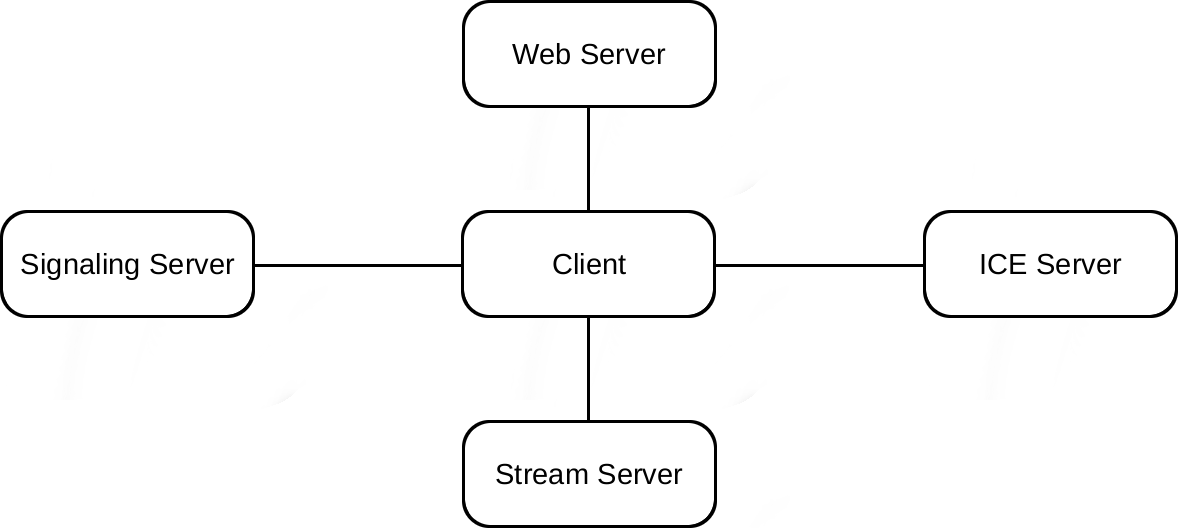
\includegraphics[width=0.6\textwidth]{figures/archs.png}
	\caption{System Modules}
        \label{fig:modules}
\end{figure}
%RP as figuras têm de ser apresentadas. Figure~\ref{fig:modules} presents ...
Figure~\ref{fig:modules} presents the structure of our system which is divided into five modules. 

 The Web Server sends Web Pages, containing the other modules information, to the client, after this, the client contacts all the other modules. The \ac{ICE} server will be used for \ac{NAT} traversal. The Stream Server will be used to record streams for further playback. The signaling server will be responsible for user and calls management and presence information. The web server will provide libraries to the client in order to interact with the other modules.

Clients can discover chat rooms and other clients by querying the signaling server, they can create rooms for multi-party communication which is achieved by using \ac{WebRTC}'s \emph{MediaStream} and \emph{DataChannel}, namely for audio, video and text communication.

Chat rooms can be public or private. Public chat rooms are moderated by a group of clients which initially is formed by the room creator, this type of room has no access restrictions by default, but that can be changed by its moderators. Private chat rooms will be visible for a list of clients or can be accessed by clients that have a link for that chat room.

Each room will be associated to multiple Media-Types, interactive and non-interactive, discrete and continuous. This media types can be structured with chains of events. Some components of the user interface may not be synchronized to all participants, for example an help or suggestion window.  

 %RP não queres falar da comunicação com outros peers?
 %RP há conversas p2p ou todos os clientes ligam ao stream server? Acho que podes dar mais detalhes nesta fase

 %RP antes de passar para a implementação deves falar em maior detalhe destes componentes. Como interagem entre si. Qual a informação que cada um guarda troca com os outros.
 %RP quais os requisitos de tecnologia para cada componente.
 %RP precisas de fornecer muitos mais detalhes. A arquitectura deverá ter várias páginas. A tua ainda só tem meia e passas logo para a implementação do protótipo.
 
\subsection{Implementation Proposal}
The infrastructure is composed by: Ice Server, Web Server, Stream Server, Signaling Server and Test Clients.

\begin{figure}[H]
	\centering
	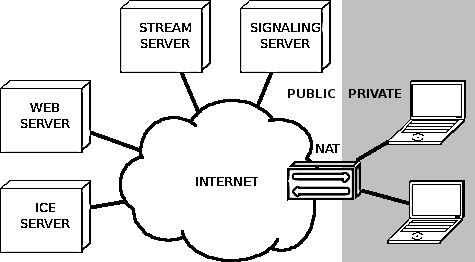
\includegraphics[width=0.6\textwidth]{figures/arch.png}
	\caption{System Infrastructure}
\end{figure}

Although the core infrastructure is important and crucial for the implementation of our web application, there is no preference for a specific software running on the web server. An important requirement for the Web Server is the WebSockets support, The \emph{LAMP} stack was considered, although the chosen technology for web development is the \emph{Play Framework} with \emph{Java}, which has a more evident separation between \emph{Model}, \emph{View} and \emph{Controller} components.

For the signaling server there is also no preference between \ac{SIP} and \ac{XMPP}, as both support presence information feature. \ac{SigOfly} could be adopted as well, but using it would be irrelevant for the final result of this project. For the sake of simplicity and easy deployment, the chosen platform is the \emph{Ejabberd} \ac{XMPP} application server, since it implements \cite{xep0206} which is crucial for web applications. \emph{Ejabberd}, as said before, is also the \ac{XMPP} server that implements more extensions. Initially, for simplicity, \emph{Ejabberd} will be configured as a single node instead a member of a cluster. 

The streaming server will be the \emph{Jitsi Videobridge} as the \emph{Jitsi} team is working with \ac{WebRTC} and their code is open source.

The \ac{ICE} server is not required to be on our infrastructure, as a public \ac{ICE} server could be used. If \ac{TURN} is used, the network speed could drop due to resource sharing with other users. An \ac{ICE} server will be installed in order to prevent the influence of other users on our application.

On the client computers, both \emph{Mozilla Firefox} and \emph{Google Chrome} will be installed as web browsers. Libraries such as \emph{jQuery}, \emph{Bootstrap}, \emph{Strophe}, \emph{Modernizr} and \emph{TogetherJS} will be downloaded from the Web Server and executed on the client side.

\begin{figure}[H]
	\centering
	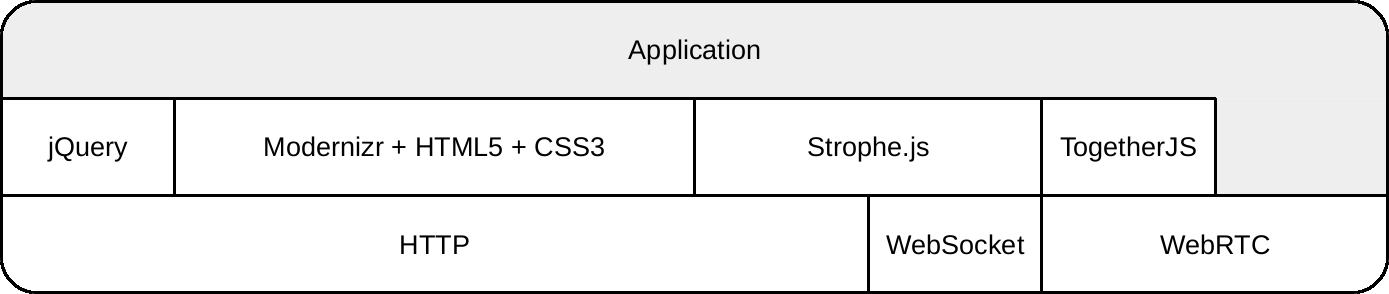
\includegraphics[width=0.95\textwidth]{figures/apparch.png}
	\caption{App Architecture}
	        \label{fig:apparch}

\end{figure}
%RP apresentar figura
Figure~\ref{fig:apparch} presents the application architecture and the underlying technologies. \emph{Modernizr} and \emph{jQuery} will ensure that our application is compatible with the most popular web browsers.
\emph{Bootstrap} will be used to make the user interface more appellative and responsive. With \emph{Bootstrap} it is quite easy to develop applications that adapt to mobile devices with different screen sizes.
The \emph{Strophe} library will be essential to communicate with the \ac{XMPP} server.
%RP era este o sentido da frase? Ou entre cliente e servidor apenas?


\emph{TogetherJS} will be used for the collaborative component of our web application. Other libraries were considered but, as said before, \emph{TogetherJS} does not provide object storage giving us the ability to choose how to store collaborative objects. We assume that \emph{JavaScript} objects are enough for implementing our application but \emph{TogetherJS} provides the flexibility to change our storage model.
%RP relê a frase. É mesmo isto que queres dizer? ``does not implement''

The synchronization between multimedia elements will be performed trough chains of \emph{JavasSript} events, other animations can be implemented with \ac{SVG} embedded on \ac{HTML}.
%RP já não vais usar smil? Como fazes a sincronização. Explica, sff.
